\section{Improving Convergence Speed}

A good optimization algorithm is esential for fitting a deep neural network, however the convergence rate can often be improved by modifying the network aritecture itself such that the cost function is easier to optimize. These modifications does not radically alter the network, but rather modifies existing layers. The modifications can also become the idendity function though parameter optimization and thus doesn't change the theoretical capabilities of the neural network.

\subsection{Batch Normalization}
Traditionally in feed forward neural networks it has been the norm to standarize the input to have zero mean and unit variance.
\begin{equation}
\hat{\mathbf{x}} = \frac{\mathbf{x} - \mathbb{E}[\mathbf{x}]}{\sqrt{\textsc{Var}[\mathbf{x}]}}
\end{equation}

This standaridization places the input to the sigmoid activation function in its linear domain ($\sigma(\epsilon) \approx \epsilon, \forall \epsilon \in [-1, 1]$), which is a reasonable starting point for the optimization \todo{[LeCun et al., 1998b; Wiesler \& Ney, 2011]}. Batch normalization extends this idea to standardize before all activation functions in a deep neural network. This has positive consequences beound limiting the sigmoid activation to its linear domain \cite{batch-normalization}.

Consider a neural network with just one hidden layers:
\begin{equation}
\mathcal{L}(\mathbf{y}, \mathbf{W}_2 \sigma(\mathbf{W}_1 \mathbf{x} + \mathbf{b}_1) + \mathbf{b}_2)
\end{equation}
where $\sigma$ is the activation function. When optimizing the loss function, the parameters $\mathbf{W}_1, \mathbf{W}_2, \mathbf{b}_1$ and $\mathbf{b}_2$ are all optimized simultaneously. The optimization of $\mathbf{W}_2, \mathbf{b}_2$ does directly depend on $\sigma(\mathbf{W}_1 \mathbf{x} + \mathbf{b}_1)$ though the error term. This becomes and issue when the distribution of $\sigma(\mathbf{W}_1 \mathbf{x} + \mathbf{b}_1)$ changes, because the updated $\mathbf{W}_2$ and $\mathbf{b}_2$ assumes the original distribution. This change of the distribution of the internal activations is called an \textit{internal covariate shift}. \cite{batch-normalization}.

The \textit{internal covariate shift} issue can be ilustrated by considering a scalar $a = w x + b \sim \mathcal{N}(b, w)$ as it would appear in a very simple neural network, and then apply sigmoid activation function on $\mathcal{N}(b, w)$ by using the \textit{change of variable theorem}. Using this one can change $w$ and $b$ and observe how the sigmoid activation distribution changes (Figure \ref{fig:batch-norm-activation-distribution}).

\begin{figure}[h]
	\centering
	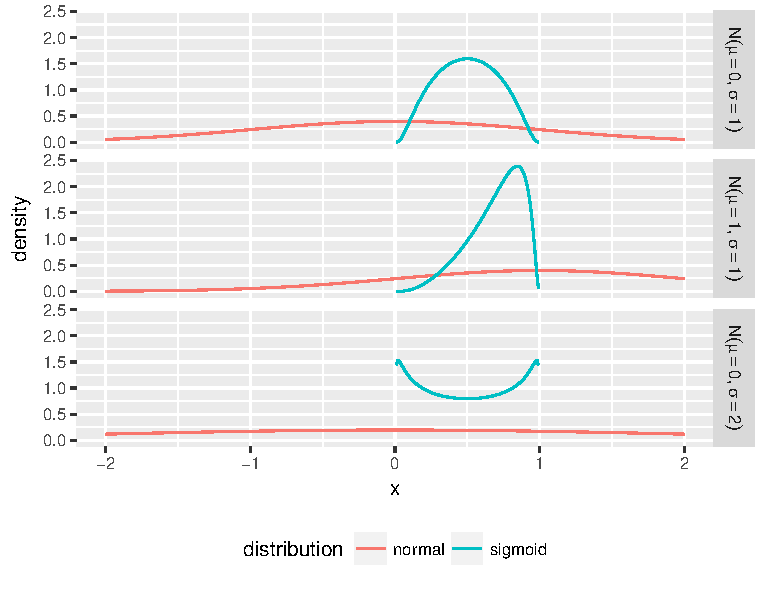
\includegraphics[scale=1]{theory/batch-norm-activation-distribution}
	\caption{Shows $X \sim \mathcal{N}(\mu, \sigma)$ and $\mathrm{sigmoid}(X)$ calculated using the \textit{change of variable theorem}.}
	\label{fig:batch-norm-activation-distribution}
\end{figure}

Batch Normalization solves this issue by standardizing the input to the activation function. To truly standardize this input the convariance matrix as well as its inverse square root should be calculated. This is very expensive thus Batch Normalization makes a pratical compromise by only standardizing using the variance.
\begin{equation}
\hat{\mathbf{a}} = \frac{\mathbf{a} - \mathbb{E}[\mathbf{a}]}{\sqrt{\textsc{Var}[\mathbf{a}]}}, \mathbf{b} = \sigma(\hat{\mathbf{a}})
\end{equation}

The expectation and variance themself are expensive to estimate over the entire dataset, thus it's only done over each mini-batch. This also makes it much more feasable to integrate the standardization into the backpropergation itself.

Finally to allow Batch Normalization to become the indendity function, two more parameters are added to the optimzation:
\begin{equation}
\hat{\mathbf{a}} = \bm{\gamma} \frac{\mathbf{a} - \mathbb{E}[\mathbf{a}]}{\sqrt{\textsc{Var}[\mathbf{a}]}} + \bm{\beta}, \mathbf{b} = \sigma(\hat{\mathbf{a}})
\end{equation}

\subsection{Residual Learning}
\cite{residual-learning}

\subsection{Layer Normalization}
\cite{layer-normalization}
